\documentclass[12pt]{article}
\usepackage{fancyhdr}
\usepackage[letterpaper, margin=1in]{geometry}
%\usepackage{indentfirst}
\usepackage{graphicx}
\usepackage{amsmath}
\usepackage{amssymb}
\usepackage{siunitx}
\sisetup{detect-weight=true, detect-family=true} % makes siunitx follow font formatting like bold, italic, etc.
\usepackage{cancel}
\usepackage{isotope}
\usepackage{listings}
\usepackage[dvipsnames,table]{xcolor}
\usepackage{xspace}
\usepackage{booktabs} % makes tables pretty
\usepackage{longtable} % for long tables
\usepackage{multirow} % makes tables pretty
\usepackage{multicol} % makes tables pretty
\usepackage{setspace}
\usepackage{subcaption}
\usepackage{hyperref}
\usepackage{cleveref}
\newcommand{\creflastconjunction}{, and\nobreakspace} % adds oxford comma to cleveref
\usepackage[utf8]{inputenc}
\usepackage{textcomp}
\usepackage{titlesec}
\usepackage{svg}
\usepackage{pdflscape} % makes pages landscape
\usepackage{mathtools}
\usepackage{enumitem}
\usepackage[T1]{fontenc}




% si units stuff
\DeclareSIUnit\year{yr}
\DeclareSIUnit\hour{hr}
\DeclareSIUnit\mole{mol}

% fancy header stuff
\usepackage{fancyhdr}
\pagestyle{fancy}

\setlength{\headheight}{28pt}
\lhead{NSE 565 \\ Winter 2022}
\chead{Homework 1\\}
\rhead{Austin Warren\\Due February 11, 2022}

% bib if needed
\bibliographystyle{ieeetr}

\begin{document}

%%%%%%%%%%%%%%%%%%%%%%%%%%%%%%%%%%
\section{Methods}


%%%%%%%%%%%%%%%%%%%%%%%%%%%%%%%%%%
\section{Results}
    % plots
    \Cref{fig:case1} shows the two solutions for Case 1: 5 control volumes and $\overline{V}=\SI{0.1}{\meter\per\second}$.
    \Cref{fig:case2} shows the two solutions for Case 2: 5 control volumes and $\overline{V}=\SI{2.5}{\meter\per\second}$.
    \Cref{fig:case3} shows the two solutions for Case 3: 20 control volumes and $\overline{V}=\SI{2.5}{\meter\per\second}$.
    \begin{figure}[htbp]
        \centering
        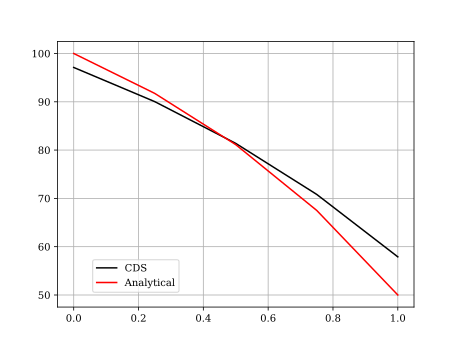
\includegraphics[width=\textwidth]{plots/graph_case1.png}
        \caption{Central Difference Scheme and Analytical Solutions for Case 1.}
        \label{fig:case1}
    \end{figure}

    
    \begin{figure}[htbp]
        \centering
        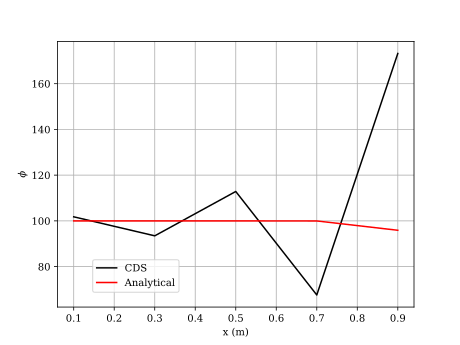
\includegraphics[width=\textwidth]{plots/graph_case2.png}
        \caption{Central Difference Scheme and Analytical Solutions for Case 2.}
        \label{fig:case2}
    \end{figure}

    
    \begin{figure}[htbp]
        \centering
        \includegraphics[width=\textwidth]{plots/graph_case3.png}
        \caption{Central Difference Scheme and Analytical Solutions for Case 3.}
        \label{fig:case3}
    \end{figure}

    \clearpage
    % table
    \Cref{tab:error} lists the error values calculated for each case.
    \begin{table}[htbp]
	 \centering
	 \caption{Error values for each case.}
	 \begin{tabular}{cc}
		 \toprule
		 Case & Error \\ 
		 \midrule 
		 1 & 0.2629491288831474 \\ 
		 2 & 26.174593696190538 \\ 
		 3 & 0.6567406338821179 \\ 
		 \bottomrule 
	 \end{tabular} 
	 \label{tab:error} 
\end{table}

    

%%%%%%%%%%%%%%%%%%%%%%%%%%%%%%%%%%
\section{Discussion}


\end{document}